\documentclass[border=5pt]{standalone}
\usepackage[utf8]{inputenc}
\usepackage{array}
\usepackage{amssymb}
\usepackage{amsmath}
\usepackage{tikz}
\usetikzlibrary{automata,arrows,positioning,calc}

\tikzset{auto shift/.style={auto=right,->,
to path={ let \p1=(\tikztostart),\p2=(\tikztotarget),
\n1={atan2(\y2-\y1,\x2-\x1)},\n2={\n1+180}
in ($(\tikztostart.{\n1})!1mm!270:(\tikztotarget.{\n2})$) -- 
($(\tikztotarget.{\n2})!1mm!90:(\tikztostart.{\n1})$) \tikztonodes}}}

\begin{document}
\nopagecolor
\begin{tabular}[t]{c b{2in}}
    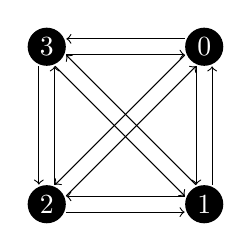
\begin{tikzpicture}
        \node[circle, inner sep=2pt, fill] (0) at (1, 1) {\color{white} 0};
        \node[circle, inner sep=2pt, fill] (1) at (1, -1) {\color{white} 1};
        \node[circle, inner sep=2pt, fill] (2) at (-1, -1) {\color{white} 2};
        \node[circle, inner sep=2pt, fill] (3) at (-1, 1) {\color{white} 3};
        
        \draw (0) edge[auto shift] (1)
              (1) edge[auto shift] (0)
              
              (0) edge[auto shift] (2)
              (2) edge[auto shift] (0)
              
              (0) edge[auto shift] (3)
              (3) edge[auto shift] (0)
              
              (1) edge[auto shift] (2)
              (2) edge[auto shift] (1)
              
              (1) edge[auto shift] (3)
              (3) edge[auto shift] (1)
              
              (2) edge[auto shift] (3)
              (3) edge[auto shift] (2);
    \end{tikzpicture}
    & This is a directed version of $\mathcal{K}_4$. \\ \\
    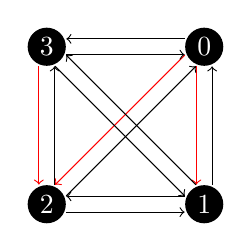
\begin{tikzpicture}
        \node[circle, inner sep=2pt, fill] (0) at (1, 1) {\color{white} 0};
        \node[circle, inner sep=2pt, fill] (1) at (1, -1) {\color{white} 1};
        \node[circle, inner sep=2pt, fill] (2) at (-1, -1) {\color{white} 2};
        \node[circle, inner sep=2pt, fill] (3) at (-1, 1) {\color{white} 3};
        
        \draw (0) edge[auto shift, color=red] (1)
              (1) edge[auto shift] (0)
              
              (0) edge[auto shift, color=red] (2)
              (2) edge[auto shift] (0)
              
              (0) edge[auto shift] (3)
              (3) edge[auto shift] (0)
              
              (1) edge[auto shift] (2)
              (2) edge[auto shift] (1)
              
              (1) edge[auto shift] (3)
              (3) edge[auto shift] (1)
              
              (2) edge[auto shift] (3)
              (3) edge[auto shift, color=red] (2);
    \end{tikzpicture}
    & Suppose the directed minimum spanning tree sampled from the graph, $\vec{T}^*$, is shown in red.\\ \\
    & Next set the node demands equal to $\deg^+\vec{T}^* - \deg^+\vec{T}^*$ for each node and find the minium cost flow. \\ \\
    & In this case the demands are 
    \begin{itemize}
        \setlength\itemsep{0mm}
        \item $0 \rightarrow 2$
        \item $1 \rightarrow -1$
        \item $2 \rightarrow -2$
        \item $3 \rightarrow 1$
    \end{itemize} \\ \\
    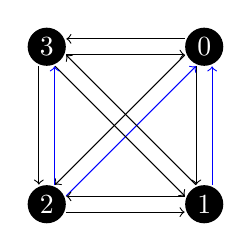
\begin{tikzpicture}
        \node[circle, inner sep=2pt, fill] (0) at (1, 1) {\color{white} 0};
        \node[circle, inner sep=2pt, fill] (1) at (1, -1) {\color{white} 1};
        \node[circle, inner sep=2pt, fill] (2) at (-1, -1) {\color{white} 2};
        \node[circle, inner sep=2pt, fill] (3) at (-1, 1) {\color{white} 3};
        
        \draw (0) edge[auto shift] (1)
              (1) edge[auto shift, color=blue] (0)
              
              (0) edge[auto shift] (2)
              (2) edge[auto shift, color=blue] (0)
              
              (0) edge[auto shift] (3)
              (3) edge[auto shift] (0)
              
              (1) edge[auto shift] (2)
              (2) edge[auto shift] (1)
              
              (1) edge[auto shift] (3)
              (3) edge[auto shift] (1)
              
              (2) edge[auto shift, color=blue] (3)
              (3) edge[auto shift] (2);
    \end{tikzpicture}
    & This is the min flow returned from \verb|min_cost_flow|. \\ \\
    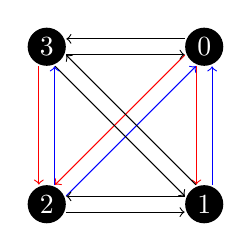
\begin{tikzpicture}
        \node[circle, inner sep=2pt, fill] (0) at (1, 1) {\color{white} 0};
        \node[circle, inner sep=2pt, fill] (1) at (1, -1) {\color{white} 1};
        \node[circle, inner sep=2pt, fill] (2) at (-1, -1) {\color{white} 2};
        \node[circle, inner sep=2pt, fill] (3) at (-1, 1) {\color{white} 3};
        
        \draw (0) edge[auto shift, color=red] (1)
              (1) edge[auto shift, color=blue] (0)
              
              (0) edge[auto shift, color=red] (2)
              (2) edge[auto shift, color=blue] (0)
              
              (0) edge[auto shift] (3)
              (3) edge[auto shift] (0)
              
              (1) edge[auto shift] (2)
              (2) edge[auto shift] (1)
              
              (1) edge[auto shift] (3)
              (3) edge[auto shift] (1)
              
              (2) edge[auto shift, color=blue] (3)
              (3) edge[auto shift, color=red] (2);
    \end{tikzpicture}
    & Add the support of $\vec{T}^*$ and the min flow \\
\end{tabular}
\end{document}
